\documentclass[border=10pt]{standalone}
\usepackage{tikz}
\usetikzlibrary{arrows.meta, shapes, calc}

\begin{document}
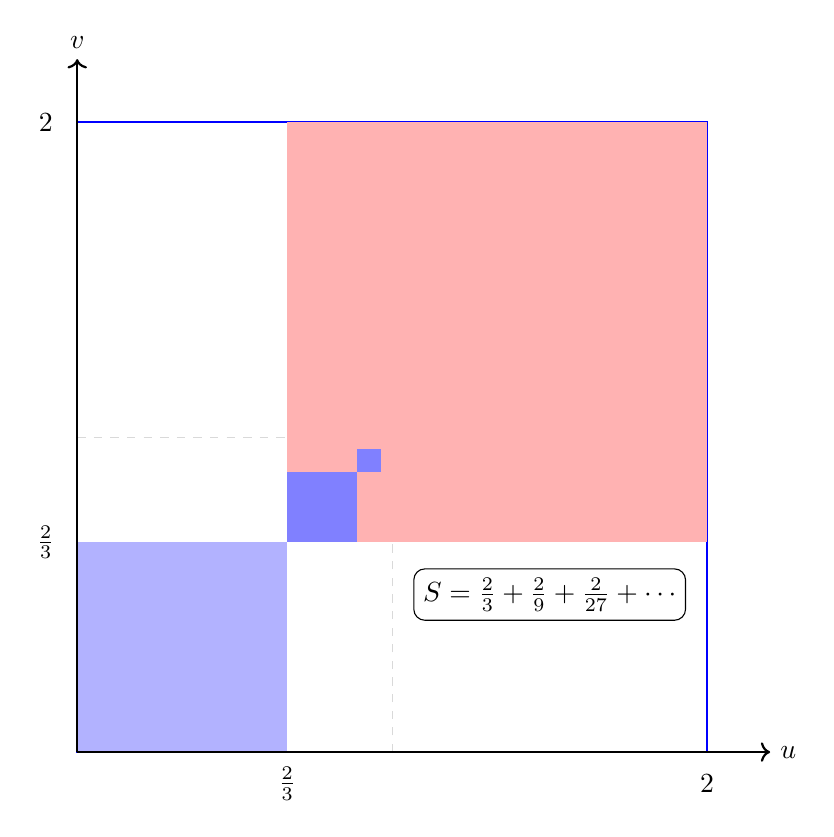
\begin{tikzpicture}[scale=4]
    % Grid
    \draw[help lines, color=gray!30, dashed] (0,0) grid (2,2);
    
    % Main square
    \draw[thick, color=blue] (0,0) rectangle (2,2);
    
    % Bottom-left quadrant
    \fill[blue!30] (0,0) rectangle (2/3,2/3);
    
    % Top-right quadrant
    \fill[red!30] (2/3,2/3) rectangle (2,2);
    
    % Series terms
    \fill[blue!50] (2/3,2/3) rectangle (2/3 + 2/9,2/3 + 2/9);
    \fill[blue!50] (2/3 + 2/9,2/3 + 2/9) rectangle (2/3 + 2/9 + 2/27,2/3 + 2/9 + 2/27);
    
    % Axes
    \draw[->, thick] (0,0) -- (2.2,0) node[right] {$u$};
    \draw[->, thick] (0,0) -- (0,2.2) node[above] {$v$};
    
    % Axis labels
    \node at (2/3,-0.1) {$\frac{2}{3}$};
    \node at (2,-0.1) {$2$};
    \node at (-0.1,2/3) {$\frac{2}{3}$};
    \node at (-0.1,2) {$2$};
    
    % Series formula
    \node[draw, fill=white, rounded corners] at (1.5,0.5) {$S = \frac{2}{3} + \frac{2}{9} + \frac{2}{27} + \cdots$};
\end{tikzpicture}
\end{document}